\chapter{Background}
This project is focused on computer vision for detecting and tracking humans in the surroundings, estimating their trajectories and distance from the PWU, the reactive control systems that prevent collisions with the detected objects as well as the augmented reality display to provide visual cues to the PWU.

\section{Human Detection}
Human detection is a subset of the classic computer vision problem of object detection. In order to develop an augmented reality system that will help PWUs to navigate in public spaces, it is essential for the system to be able to discern humans from the surroundings.

\subsection{Definition of Requirements}
 The problem arises in crowded areas, whereby individuals are occluded by other people or objects in front of them, leaving only certain body parts visible. As such, we began our research with the problem of being able to detect people in images where identifiying parts of the body are not always visible.

\subsection{Review of Existing Methodologies}
A related field of research is that of people counting and human detection in visual surveillance in public areas. Where the problem differs is that surveillance benefits from being able to rely on cameras with a good view of the crowd from above, whereas for a PWU, the camera will not have as high of a vantage point, making detecting every single individual in a crowd impossible. 

Despite the disadvantage, similar techniques can be used to detect humans in video. Most methods can be classified into two categories \cite{Hou2010}. The first technique, foreground detection, attempts to model the background of an image and then detect the changes that occur between frames. The second category involves exhaustively searching the image with a scanning window, and deciding if each window can be classified into a human shape.

\begin{figure}[ht]
	\begin{subfigure}[b]{.5\textwidth}
		\centering
		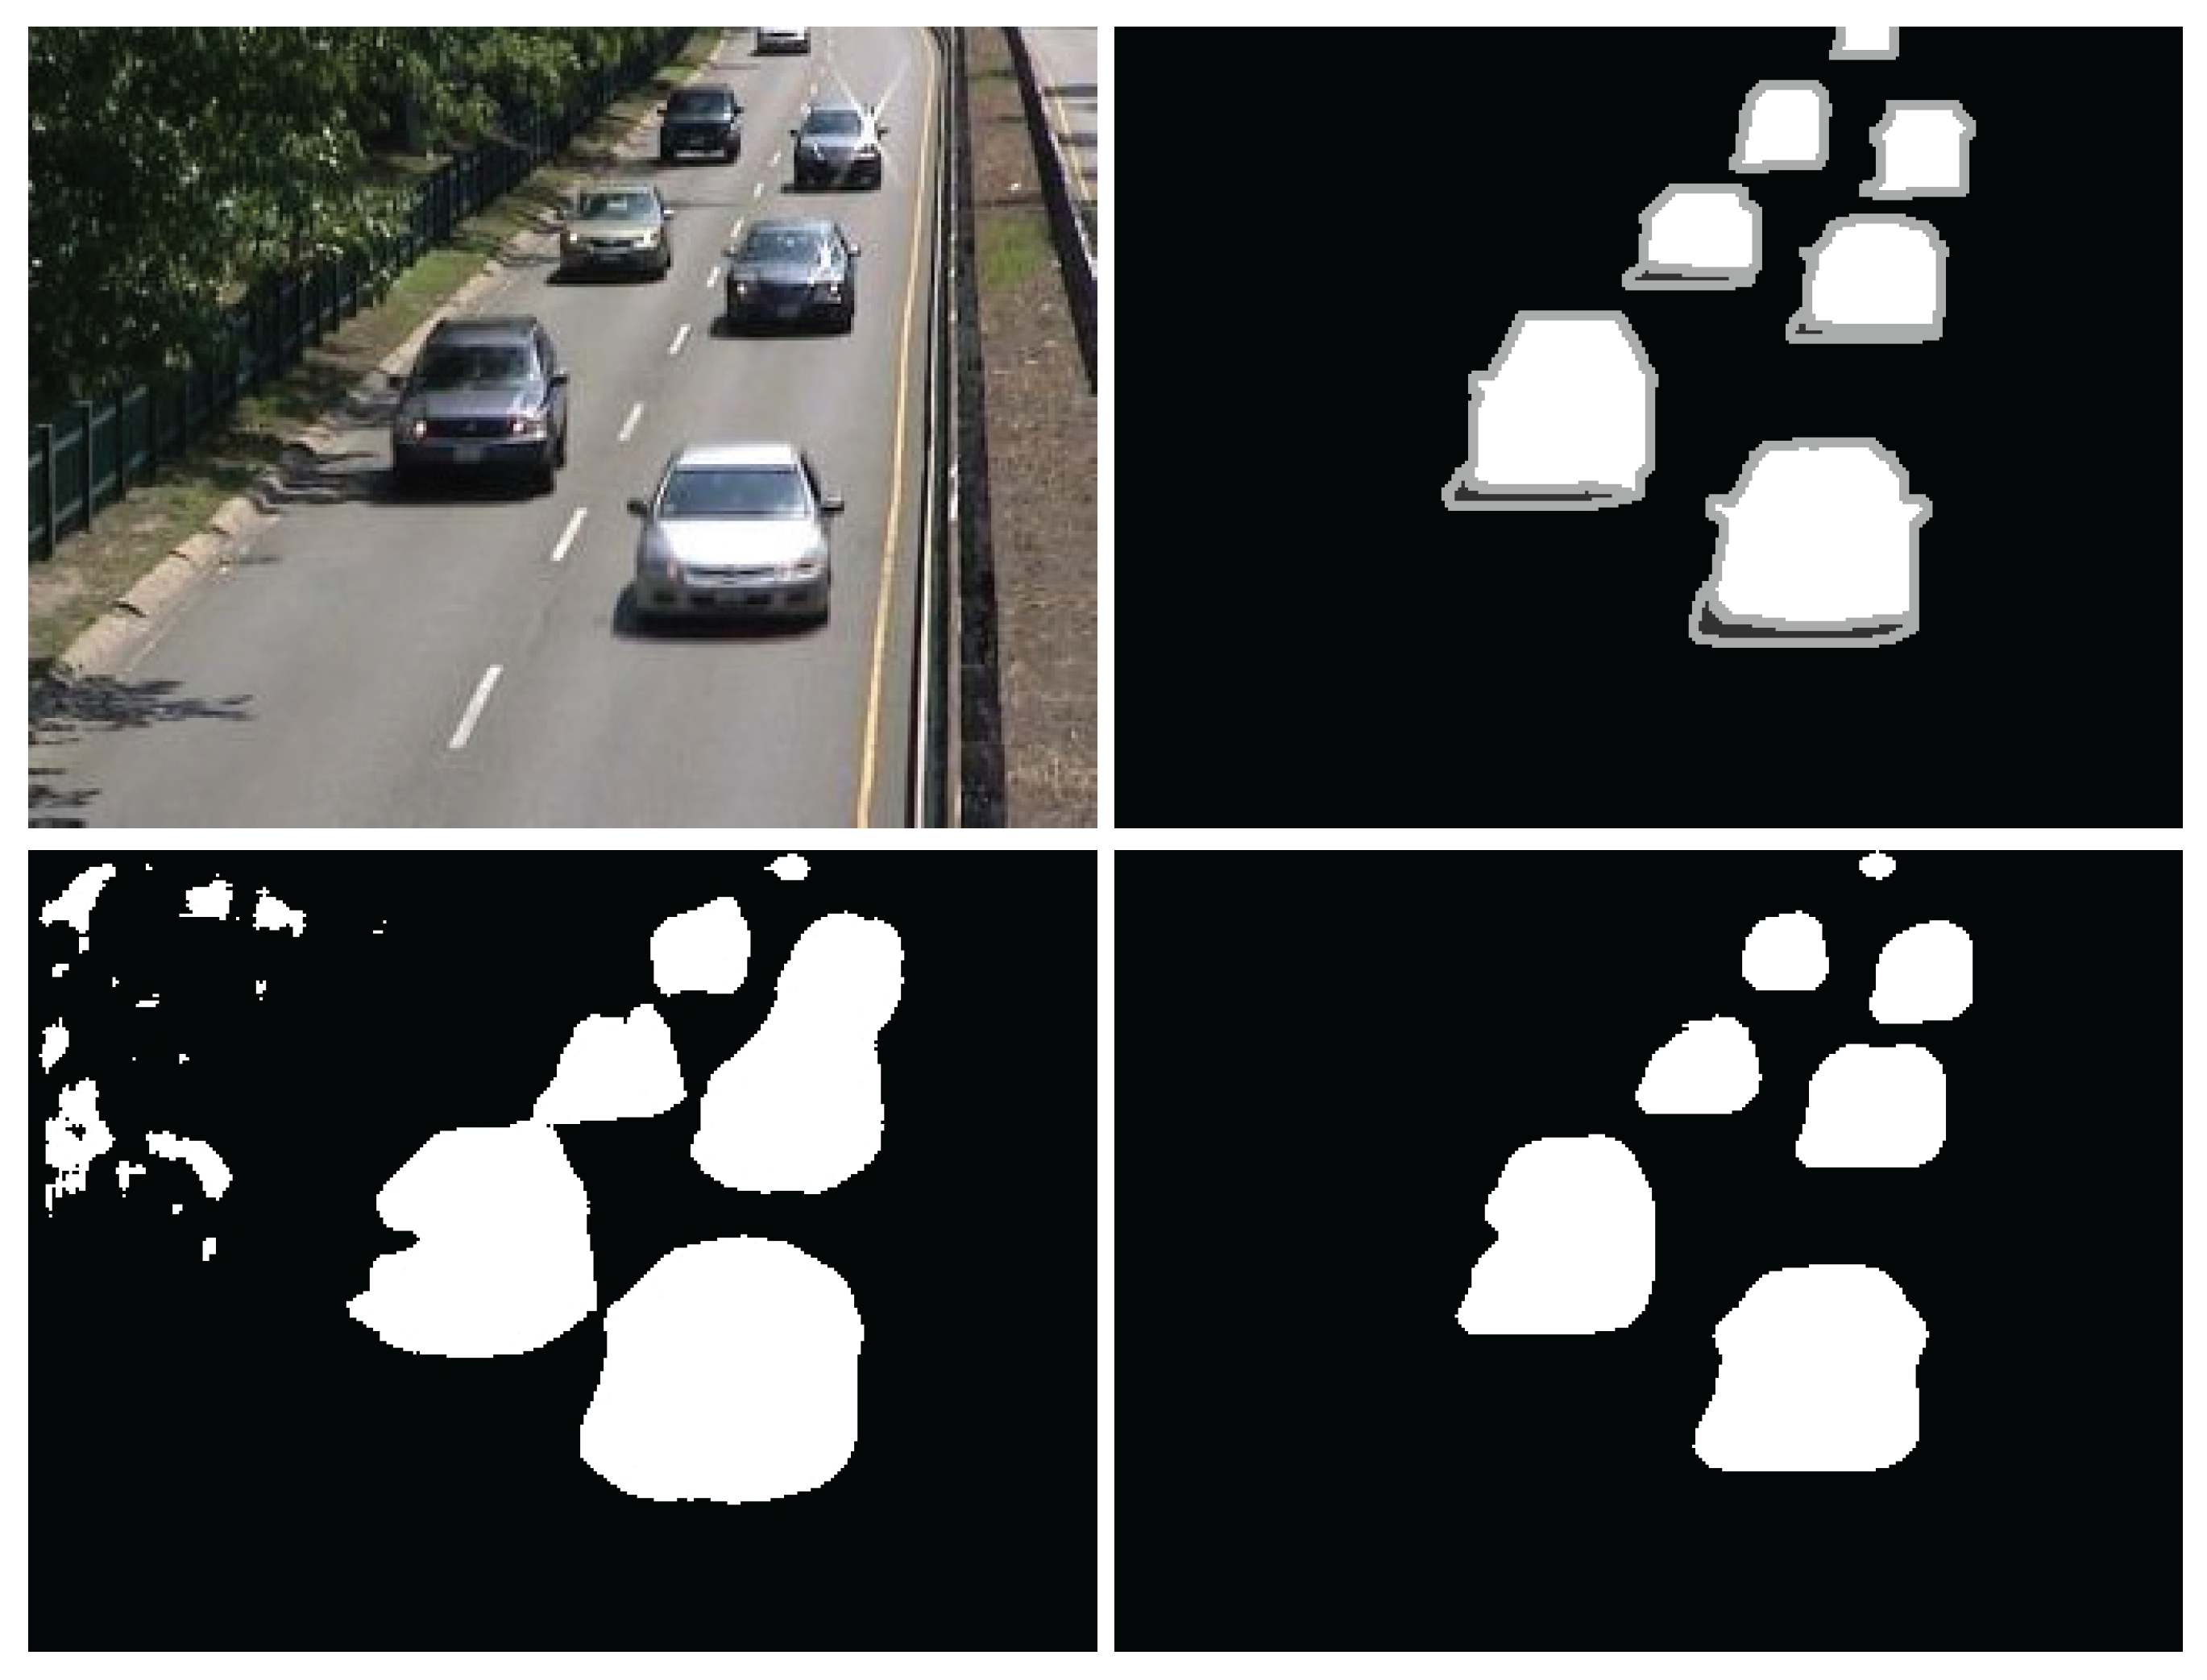
\includegraphics[width=.9\linewidth]{img/chapter2_background/robustBackgroundSubtraction.png}
		\caption{Foreground Detection \cite{Zeng2017}}
	\end{subfigure}%
	\hspace{\fill} 
	\begin{subfigure}[b]{.5\textwidth}
		\centering
		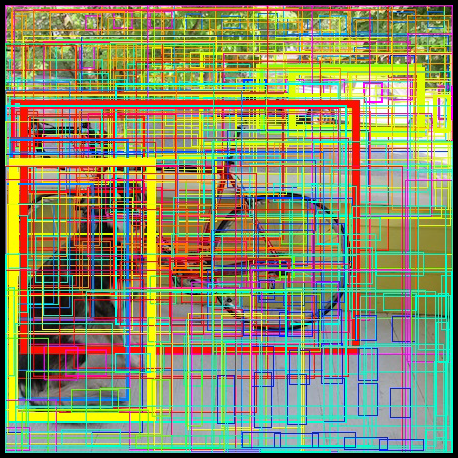
\includegraphics[width=.675\linewidth]{img/chapter2_background/yoloBBBoxes.png}
		\caption{Scanning Window \cite{Redmon}}
	\end{subfigure}
	
	\begin{center}
		\caption{Comparison of Foreground Detection and Scanning Windows}
		\label{fig:foregroundVsScanning}
	\end{center}
\end{figure}

\subsubsection{Foreground Detection}
Background subtraction is a widely used approach for detecting moving objects \cite{Piccardi2004}. A temporal average filter can be used to find the median of all the pixels in an image to form a reference image. Frames with moving objects can then be compared pixelwise to the reference, and a threshold set to determines if the pixel is part of the background or foreground. People counting and human detection can then be achieved by segmenting the foreground image into individuals.

\paragraph{} However, this technique relies on a static camera in a well placed location. This brings up several reasons as to why this method would not be suitable for this project. Firstly, the camera available is part of a head-mounted augmented reality device. The wearer has the ability to move the camera in 6 degrees of freedom. Secondly, the wearer will also be navigating a powered wheelchair. As a result, the background is constantly changing, and the reference image would require constant recomputation before human detection can even begin.

\subsubsection{Scanning Windows}
Due to the ever-changing surroundings of a mobile robot, a better approach for object detection is to exhaustively search an image using scanning windows and determining if an object was detected in each window. However, it must be noted that this method is computationally expensive. In order to achieve real-time detection on a mobile robot, the use of a graphics processing unit (GPU) should be considered \cite{Hirabayashi}.

\subsubsection{Classical Object Detection}

\paragraph{Haar Cascades}
Haar cascades classifies images based on the value of simple features \cite{Viola2001}, which are variants of the difference between the sum of pixel values in rectangular regions. An intermediate representation of the original image is used to rapidly compute a small set of representative rectangular features.

\paragraph{}A cascade of classifiers is then used to determine if the region is detected as a human. The detection process is that of a degenerate decision tree, where a positive result in the first cascade will trigerr an evaluation in the second, more successful classifier. As such, the initial classifier can eliminate a large number of negative examples with very little processing. After several stages, the number of sub-windows has been reduced radically

\paragraph{Histograms of Oriented Gradients}
The method proposed is implemented by dividing the image window into small spatial regions and calculating a local 1-D histogram of gradient directions for all the pixels in the region. The combined local histograms form the overall feature representation of the image.

\paragraph{}The detection window is tiled with the Histogram of Oriented Gradient (HOG) descriptors. In the original paper \cite{Dalal2005}, these feature vectors were then used in a conventional SVM based window classifier  to give human detections.

\subsubsection{Deep Learning Object Detection}
Modern approaches for human detection largely depend on Deep Convolutional Neural Networks (CNN). The approach provides the best in class performance, as well as scaling effectively with more data. An added advantage of using CNN based object detection systems for this project is that they are also capable of detecting multiple classes of objects.

\paragraph{}An issue with CNN approaches is that the methods are trying to draw bounding boxes around objects of interest in images. However, we do not know the number of objects in the image beforehand. As such, to be completely sure every object has been detected, a naive solution is to take a huge number of regions and attempt to classify all the objects in the region, a computationaly expensive process.

\begin{figure}[ht]
	\centering
	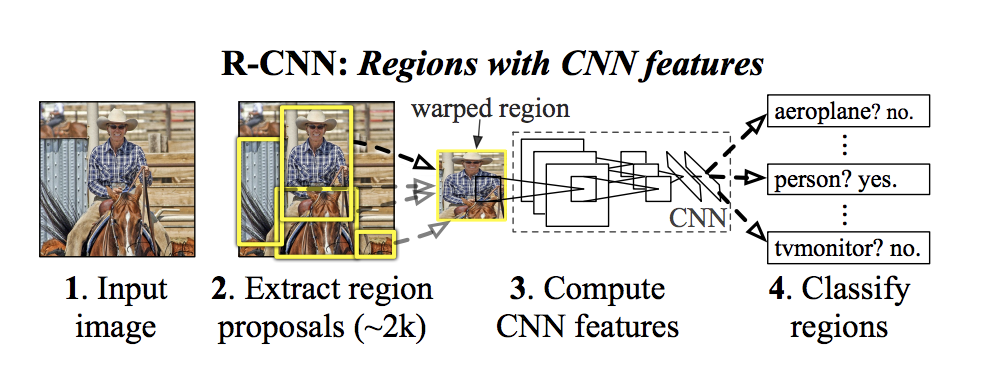
\includegraphics[width=.9\linewidth]{img/chapter2_background/rcnn.png}
	\caption{R-CNN Approach}
\end{figure}

\paragraph{R-CNN} The R-CNN method uses a selective search to extract 2000 regions from an image \cite{Girshick2014}. The regions are selected by generating a large number of candidate regions and using a greedy algorithm to recursively combine similar regions into larger ones. The regions are then fed into a CNN that acts as a feature extractor and the output dense layer consists of the features extracted from the image, which are then fed into an SVM to classify the presence of objects in the region.

\paragraph{}The major disadvantage to this approach is the amount of time required to train the network. Each training image has to be classied once for each of the 2000 region proposals. Furthermore, the selective search algorithm is a fixed algorithm (no learning is done), and as such, could lead to generation of bad candidate region proposals.

\paragraph{YOLO} Whereas R-CNN uses regions to localize the object within an image, You Only Look Once (YOLO) looks at the image as a whole and uses a single CNN to predict the bounding box and the class probabilities \cite{Redmon}. By looking at the image as a whole, the network can use features from the entire image to predict each bounding box.

\begin{figure}[ht]
	\centering
	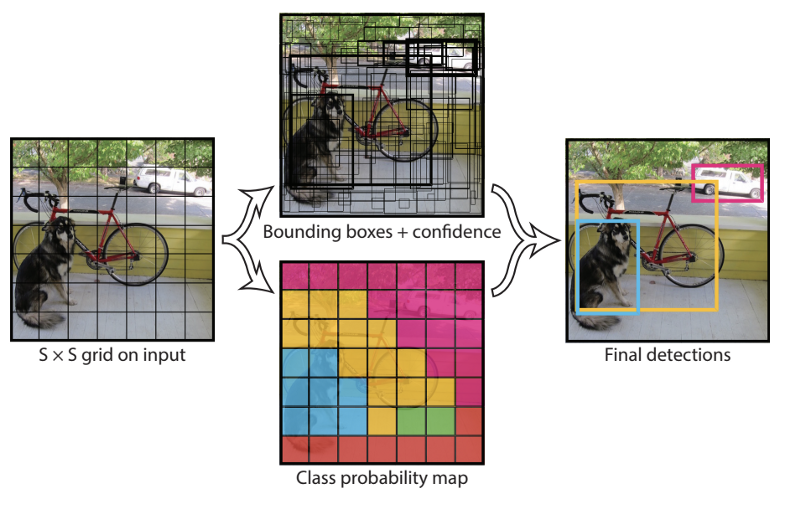
\includegraphics[width=.6\linewidth]{img/chapter2_background/yoloApproach.png}
	\caption{YOLO Approach}
\end{figure}

The model divides the image into an $S \times S$ grid, and for each cell, predicts a number of bounding boxes, the confidence for those boxes and the class probabilities.

\subsection{Comments}
As seen from the research, we can clearly see that there are many ways to solve the human detection problem. The classical approaches, although computationally efficient, are siginficiantly outperformed by the deep learning approaches. For a mobile robot in a public area, we want to be able to detect almost all humans in the surroundings to better inform the PWU.

\paragraph{}However, the major disadvantage of the deep learning approach is the time taken to train the network, as well as the requirement of a GPU to achieve real-time performance. These issues will be addressed in a later section of the report.

\section{Object Tracking}
% Object tracking
% Track objects across frame to get a sense of direction

\section{Head Pose Estimation}

\section{Body Pose Estimation}
% Human body pose estimation
% The pose of the shoulders and body can be used to determine the direction

\section{SLAM}

\section{Augmented Reality Headsets}